%
\documentclass[hdr, oneside, final]{unswthesis}
\usepackage{mystyle} % all include packages and definitions
\usepackage{lipsum}
\usepackage{siunitx}
\usepackage{amsmath}
\usepackage{authblk}
\usepackage{verbatim}
\usepackage{xcolor}

\definecolor{codegreen}{rgb}{0,0.6,0}
\definecolor{codegray}{rgb}{0.5,0.5,0.5}
\definecolor{codepurple}{rgb}{0.58,0,0.82}
\definecolor{backcolour}{rgb}{0.95,0.95,0.92}

\lstdefinestyle{mystyle}{
    backgroundcolor=\color{backcolour},   
    commentstyle=\color{codegreen},
    keywordstyle=\color{magenta},
    numberstyle=\tiny\color{codegray},
    stringstyle=\color{codepurple},
    basicstyle=\ttfamily\tiny,  %set font size
    breakatwhitespace=false,         
    breaklines=true,                 
    captionpos=b,                    
    keepspaces=true,                 
    numbers=left,                    
    numbersep=5pt,                  
    showspaces=false,                
    showstringspaces=false,
    showtabs=false,                  
    tabsize=2,
    lineskip=0.1pt  %set line space
}

\lstset{style=mystyle}

\DeclareSIUnit{\sqrthz}{\ensuremath{\sqrt{\text{\hertz}}}}
\DeclareSIUnit{\voltnoise}{\volt\per\sqrthz}

\makeatletter
\fancypagestyle{noHeading}{
        \fancyhead{}
        \renewcommand{\headrulewidth}{0pt}
}
\raggedbottom

\thesistitle{Thesis Topic}
\thesisschool{School of Computer Science and Engineering}
\thesisauthor{Firstname Lastname}
\thesisZid{z1234567}
\thesisdegree{Doctor of Philosophy}
\thesisdate{November 2020}
\thesissupervisor{Firstname Lastname}% for undergrad theses only
 % Thesis details e.g. Title

\newcommand*\mean[1]{\overline{#1}}
\newcommand*{\Perm}[2]{{}^{#1}\!P_{#2}}

\DeclareGraphicsExtensions{.pdf,.jpeg,.png}
\graphicspath{{2-intro/}{3-literature/}{4-techchapter/}{5-techchapter/}{6-techchapter/}{8-appendices/}}


\newcommand\blankpage{
        \null
        \thispagestyle{empty}
        \addtocounter{page}{-1}
        \newpage
}

\begin{document}
    
    \renewcommand{\bibname}{References}
    %% pages in the ``frontmatter'' section have roman numeral page number
    \frontmatter  
    \maketitle
    
    %the forms from GRIS printed as pdf
    %\includepdf[pages=1]{1-pre/GRIS.pdf}
    %\includepdf[pages=1]{1-pre/GRIS2.pdf}
    % \afterpage{\blankpage}

    \chapter{Abstract}



An optical-electrode or "Optrode" is a recently developed nerve signal detection device. Optrodes are used in electro-optical detection systems to convert nerve signals into light signals. Compared to conventional electrode detection systems, this system has the advantages of lower electrical interference, low signal attenuation, and small volume. However, the current electro-optical systems' output noise levels are much higher compare to conventional electrode systems. This means it is harder to observe nerve activity, especially when the amplitude is small. Noise in the optrode system is mainly produced by the light source, which suggests the possibility of active noise canceling.

An active noise canceling method for the electro-optical detection system for better detection results is proposed in this project. By using a light splitter at the output of the light source, two channels of light that contain almost identical noise can be formed. By connecting the exact same optrode sensing circuit to the two channels, the noise output of the two channels is very similar. Then, by applying a nerve signal to the optrode in one channel and a zero signal to the optrode in the other channel, we get one channel to output a combination of noise and nerve signals, and the other channel to output only noise. By converting the light signals into digital signals and applying a suitable digital signal processing algorithm, the noise can be largely removed and a clean nerve signal can be recovered.

In this project, a light receiver board which converts and amplifies two channels of light to digital signals has been designed, constructed and tested.  The digitised signals from the light receiver board receiver board are passed to an FPGA development board on which an adaptive filter algorithm has been implemented to actively cancel the noise. Experiments were conducted to test the system noise floor, and the system's responses to sine wave signals and simulated cardiac signals applied to the active optrode. Results show up to a 50\% reduction of the receiver system's noise floor when the active noise cancelling was activated, thus the ability to recover very low amplitude signals.  It can also reduce the artifact caused by moving the system physically.


    \chapter{Acknowledgement}

Thanks to my supervisors A/Prof. Torsten Lehmann and Prof. Francois Ladouceur for their excellent guidance.

Thanks to everyone in the Multi-Optrode Array team for their technical support.

Thanks to my parents and friends for their financial and mental support.

    \chapter{Publications and Presentations}

\section*{List of Publications}
 
\begin{itemize}
    \item R. Yang, Y. Chen, F. Ladouceur, N. H. Lovell, A. Al Abed, and T. Lehmann, ``Active Noise Cancelling Method for An Electro-Optical Detection System,'' 2023 IEEE Nordic Circuits and Systems Conference (NorCAS), 2023, Accepted on Sept. 20, 2023.
\end{itemize}




    
    %\setcounter{tocdepth}{4}
    \tableofcontents
    %\addcontentsline{toc}{chapter}{\listfigurename}
    \listoffigures  % if required
    %\addcontentsline{toc}{chapter}{\listtablename}
    \listoftables  % if required
    %\chapter{Abbreviations}

%%cat */*.tex | grep -wo "[A-Z]\+\{2,10\}" | sort | uniq -c | awk '{print $2}'


\nomenclature{RMS}{Root Mean Square}
\nomenclature{PM}{Polarization-maintaining}
\nomenclature{RF}{Radio Frequency}
\nomenclature{PCB}{Printed Circuit Board}
\nomenclature{FPGA}{Field Programmable Gate Array}
\nomenclature{HDL}{Hardware Description Language}
\nomenclature{DSP}{Digital Signal Processing}
\nomenclature{FIR}{Finite Impulse Response}
\nomenclature{FxLMS}{Filtered-X Least Mean Squares}
\nomenclature{ANC}{Active Noise Cancelling}
\nomenclature{LMS}{Least Mean Square}
\nomenclature{LUT}{Look Up Table}
\nomenclature{IOB}{Input Output Block}
\nomenclature{IO}{Input Output}
\nomenclature{AC}{Alternating Current}
\nomenclature{DC}{Direct Current}
\nomenclature{MOSFET}{Metal-oxide-semiconductor Field-effect Transistor}
\nomenclature{EMI}{Electromagnetic Interference}
\nomenclature{DAC}{Digital-to-Analog Converter}
\nomenclature{ADC}{Analog-to-Digital Converters}
\nomenclature{SPI}{Serial Peripheral Interface}
\nomenclature{I2C}{Inter-Integrated Circuit}
\nomenclature{LDO}{Low-dropout}
\nomenclature{BCI}{Brain-computer Interface}
\nomenclature{RTL}{Register-transfer Level}
\nomenclature{USB}{Universal Serial Bus}
\nomenclature{APSoCs)}{All Programmable System-on-Chips}
\nomenclature{PC}{Personal Computer}
\nomenclature{LED}{Light Emitting Diode}
\nomenclature{SD Card}{Secure Digital Card}
\nomenclature{FIFO}{First In First Out}

\printnomenclature[5em]

 % if required
    
    %% pages in the ``mainmatter'' section have arabic page numbers and chapters are numbered
    \mainmatter
    \pagestyle{fancy}
        \fancyhf{}
        \fancyhead[LE]{\leftmark}
        \fancyhead[RO]{\rightmark}
        \fancyfoot[C]{\thepage}
        \renewcommand{\headrulewidth}{1pt}
        \setcounter{secnumdepth}{3}
   
   
    %chapters
    \chapter{Introduction}


\section{Optrode System}

\begin{figure}[htbp]
\centerline{\includegraphics[width=0.9\linewidth]{OptrodeFigure.pdf}}
\caption{(a) Diagram of optrode transducer used in electrophysiological  detection.  Light comes in from Polarization-maintaining (PM) fibre, is rotated by liquid crystal, reflected by the mirror and goes back into the PM fibre. (b) Optrode electrophysiological  detection system block diagram.  Light goes into the optrode from the light source, carries nerve signal, and is converted at the receiver board and DAQ to digital signal.}
\label{fig_OptrodeFigure}
\end{figure}

An optical-electrode or ``optrode'' is a recently developed device for detecting biopotential signals of neuronal, cardiac, or muscular origin.~\cite{OptrodeTransducer}.  Fig.~\ref{fig_OptrodeFigure}(a) shows the structure of such an optrode: light that is generated from a super-luminescent diode light source is guided to the optrode via a polarisation-maintaining fibre (PM fibre).  The polarised light sees its polarisation being rotated by a thin (5\ $\mu$m) layer of liquid crystals by an angle depending on the voltage applied across the metal contacts~\cite{LCVsensor}.  The light is then reflected by the back mirror and returns to the PM fibre where the amount of light recaptured depends on the rotation angle of the liquid crystals. The optrode is designed to create a linear relationship between the light detected and the voltage applied to the metal contacts.

In an existing electrophysiological  detection system such as sketched in Fig.~\ref{fig_OptrodeFigure}(b), the optrode is used to convert neuronal signals into light signals as explained above.  The light intensity recaptured is -- in this case -- modulated by the biopotential signal present at one of the metal contacts (the other one being grounded). The light that comes out from the optrode is then directed to a receiver board where a photodiode converts the light into an analogue electrical signal which is then sampled by the data acquisition equipment.

This system has lower signal attenuation~\cite{OptrodeArray,ImpedanceOfOptrode} compared to conventional electronic detection systems. However, the output noise level of the current system is significantly higher than that of conventional microelectrode-based systems. This means it is harder to observe nerve activity, especially when the signal amplitude is small (less than~\qty{10}{mV}).  In previous experiments, it was observed that most of the noise was coming from the light source and thus, a direct way to reduce noise is to design a low-noise current source~\cite{LowNoiseCurrentSource} to power the light source.  In this paper, we propose an additional method to reduce noise: active noise cancelling.

The active noise cancelling technique is used in multiple applications such as noise-cancelling headphones~\cite{ANC_Headphone_1,ANC_Headphone_2}, noise-cancelling in cars~\cite{ANC_Car}, RF signal noise-cancelling~\cite{ANC_RF}, {\em etc}.  The basic principle of active noise cancelling for the sound wave is that when two waves have basically the same frequency and amplitude but opposite phases, they will cancel each other out.  In our case, we are dealing with noise in the digital signal form, which requires filtering techniques rather than just subtracting the two signals.  Wiener filters~\cite{WienerFilter} are widely used in signal processing of active noise cancelling applications {\em e.g.}\cite{ANC_Wiener_2,ANC_Wiener_3}.  Since the nerve signal that the optrode system is detecting has a similar frequency range compared to audible sound frequency, active noise cancelling with Wiener filtering should be effective here as well. Thus we propose herein such an approach which, to the best of our knowledge, has not yet been proposed elsewhere.


\section{Scope of work}

This project aims at designing a active noise cancelling system that reduces the noise level in an existing optrode measurement system. The main outcome of this project is the active noise cancelling system that consists of two board, a light receiver PCB, and an FPGA development board. The project begins with a literature review to active noise cancelling designs, and optrode.  Then we analyzes previous receiver boards and designs a new light receiver board, simulation are run and performance are tested to ensure the circuits on the board work as expected. The heart of the project lies in the development of a noise-cancelling algorithm, starting with the foundational Wiener filter. This filter is then modified and tested first in MATLAB, and then implemented in Verilog HDL, with further explorations into the usage of DSP blocks and final implementation on an FPGA platform.  Experimental sections examine the correlation between different noise signals, compare the performance of the newly designed system with existing technologies, test with sinusoidal signals on optical input, and study the artifacts introduced by physical movements and their impact on signal quality.

    \chapter{Literature Review}\label{c:literature}

\section{Optrode system}

In recent years, optrode technology has been invented and used to interface with brains.  Compared to traditional electrodes, optrode can be more precise, take less tissue damage \cite{MoreOptrode_5}, and be able to simultaneously stimulate and record.  The light source of the optrode can be external \cite{MoreOptrode_6}\cite{MoreOptrode_7}, or integrated on the optrode \cite{MoreOptrode_8}\cite{MoreOptrode_2}.  As the optrodes are getting smaller, they can be manufactured into arrays \cite{MoreOptrode_1}\cite{MoreOptrode_3}, or even 3-dimensional arrays \cite{MoreOptrode_4}, which can cover a larger area or volume of tissue, enabling the study of network dynamics \cite{MoreOptrode_9} or interactions between different brain regions \cite{MoreOptrode_10}.  The size and power consumption of optrode systems can be small enough to fit in a portable device \cite{MoreOptrode_11}, which would be beneficial for brain-machine interfaces.

\subsection{Existing optrode system}
In this project, we are working on improving the noise performance of an existing optrode system \cite{OptrodeProceesings} (shown in fig.~\ref{fig_OptrodeFigure}).  A superluminescent diode emits light to a circulator, which directs the light to a liquid crystal transducer.  The transducer receives nerve activity signal from the two electrodes.  This causes the change of liquid crystal angle, which then changes the reflection rate of the light.  Therefore, the nerve activity message is modulated to the light and the light is reflected to the circulator, which then directs the light to a photodiode light detector.  This detector converts the light signal to a current signal, and eventually the current signal is converted to digital data via an amplifier circuit and data acquisition equipment. 

\section{Active noise cancelling}

\subsection{Wiener filter}

\begin{figure}[H]
\centerline{\includegraphics[scale=0.5]{3-literature/Wiener_block.pdf}}
\caption{Wiener filter block diagram}
\label{fig_Wiener_block}
\end{figure}

To reduce the noise in the system, an active noise reduction algorithm is needed.  The wiener filter is one of the choices when dealing with two channel noise reduction.  A FIR wiener filter for discrete signals \cite{WienerPaper} is shown in fig.~\ref{fig_Wiener_block}, s[n] is a noise free signal, and w[n] is s[n] plus some noise.  G(z) is the wiener filter with ai being the filter coefficients.   W[n] is inputted to the filter, and x[n] is the filter output.  e[n] is the error between x[n] and s[n].  From this diagram, it can be derived that the mean square error is as follows:
$E[e^2 [n]]=E[(x[n]-s[n])^2 ]$
After some derivatives and calculations, an equation came out:


\begin{gather} \label{eqn_WienerMatrix}
\underbrace{
    \begin{bmatrix}
    R_w[0] & R_w[1] & \dots & R_w[N] \\
    R_w[1] & R_w[0] & \dots & R_w[N-1] \\
    \vdots & \vdots & \ddots & \vdots \\
    R_w[N] & R_w[N-1] & \dots & R_w[0]
    \end{bmatrix}
}_{T}
\underbrace{
    \begin{bmatrix}
    a_0 \\
    a_1 \\
    \dots \\
    a_N
    \end{bmatrix}
}_{a}
=
\underbrace{
    \begin{bmatrix}
    R_{ws}[0] \\
    R_{ws}[1] \\
    \dots \\
    R_{ws}[N]
    \end{bmatrix}
}_{v}
\end{gather}

In eqn~\ref{eqn_WienerMatrix} the matrix T is the autocorrelation of w[n], and inside the matrix v is the cross correlation of w[n] and s[n], where both w[n] and s[n] is known.  Therefore, both matrix T and v are known, so matrix a can be calculated, which is the filter coefficients.
This method uses a noise free message signal s[n] and a noisy message signal w[n] as input, and the filter reduces the noise inside w[n].  This is different to how the noise reduction algorithm would work in this project.  From the optrode system, a noisy message signal and a pure noise signal can be extracted, while the pure noise signal is highly correlated to the noise inside the noise message signal.  To use the wiener filter, the pure noise signal can be the input w[n] and the noisy message signal can be the input s[n].  The output x[n] would be the correlated noise between the pure noise signal and the noisy message signal.  Then, subtract x[n] from s[n] to give the signal after noise reduction.
For two long discrete signals, say a 10s signal with a sampling rate of 100kHz, each signal has 1 million samples.  For matrix T, that means a 1 million times 1 million size, which takes a huge amount of computational power.  The plan is to run this algorithm on an FPGA, which cannot handle this task.  Also, it is desired to have real-time output with low latency.  The wiener filter is very hard to achieve both high noise reduction rate and low latency since the filter needs a fair number of samples to work.
In conclusion, the wiener filter is a good algorithm to start with.  however, it cannot suit all the requirements for this project, so modifications and other methods must be considered.



\subsection{ANC on audio systems}

Active noise cancelling technique is widely used in audio systems.  It can help remove noise from human ears either using a headset \cite{ANC_Headphone_10} or a larger speaker \cite{ANC_Car}.  There are a few ways to achieve noise cancelling with a headset, such as using a microphone at the outside of the headset to capture noise and feedforward \cite{ANC_Headphone_8} to algorithms to process, and output the anti-sound using the headset speaker.  Alternatively, the microphone can be placed inside the headset to feedback \cite{ANC_Headphone_5} noise sound and then cancel it with the speaker sound.  It is also very common to use both feedforward and feedback at the same time \cite{ANC_Headphone_4}.  
A lot of headset active noise cancelling processes \cite{ANC_Headphone_1}\cite{ANC_Headphone_2} are using Filtered-X Least Mean Squares (FxLMS) algorithm \cite{ANC_Headphone_7}, or the modified version of it \cite{ANC_Headphone_9}\cite{ANC_Headphone_6}.

The FxLMS algorithm is an advanced version of the standard Least Mean Squares (LMS) algorithm tailored for active noise cancelling. ANC aims to diminish unwanted noise by producing an ``anti-noise" sound wave that counteracts the undesired noise. A challenge in ANC is the secondary path between the speaker, which emits the anti-noise, and the error microphone, which gauges noise cancellation effectiveness; this path can introduce delays and distortions. The FxLMS algorithm addresses this \cite{ANC_Headphone_11} by first filtering the reference noise signal through a model of the secondary path, creating the "Filtered-X." Then, using this filtered-X signal and the error signal from the microphone, the LMS algorithm adaptively updates the filter weights to minimize the difference between the desired signal (typically silence) and the adaptive filter's output. This continuous adaptation allows the FxLMS algorithm to control noise in dynamic environments.

\section{Digital signal processing on FPGA}

\subsection{Active Noise Cancellation for In-Ear Headphones Implemented on FPGA}

\begin{figure}[h]
\centerline{\includegraphics[width=0.6\linewidth]{3-literature/ANCHeadphoneFPGA.pdf}}
\caption{Block Diagram for an active noise cancelling system}
\label{fig_ANCHeadphoneFPGA}
\end{figure}

A block diagram for active noise cancellation algorithm on FPGA \cite{ANC_Headphone_3} is shown in fig.~\ref{fig_ANCHeadphoneFPGA}.  The high-level design is basically a negative feedback control loop with inputs being reference microphone and error microphone, and output being sound data after noise reduction.  The feedback is connected to an adaptive filter that uses the filtered-x least mean square (FxLMS) algorithm.  The coefficients are calculated by the previous coefficients, input data, and feedback error signal inside a weight update controller.  It keeps updating the coefficient until the error signal goes to zero.  Inside the adaptive filter, there are 24 filter taps.  There are results showing that after the 17h filter tap, the coefficients are very close to zero.  Also, a comparison was made showing that 24 filter taps and 60 filter taps achieve the exact same noise reduction ability, while 60 filter taps have 200\% more computational complexity.  Therefore, 24 is an appropriate number of filter taps that does not use too many resources but still maintains decent noise reduce ability.  A pipeline structure is also designed to reduce the hardware resources used.  As high frequency noise can be largely reduced by passive noise control, active noise cancellation only needs to work at lower frequencies, for instance, lower than 1kHz.  Modern FPGAs can run at around 100MHz frequency, which is a lot faster than the required sound frequency.  In this case, 24 filter taps are being pipelined, which means for each sample period the filter is running 24 times to get 24 filter taps.  A single 24-Filter unit structure as well as the pipelined single-multiplier filter have been implemented to compare the resource utilization rate.  The result shows that the non-pipelined filter cost 77\% of slice look up tables (LUTs) and 425\% of bonded input output blocks (IOBs) on the FPGA, and the pipelined filter cost 13\% of slice LUTs and 34\% of bonded IOBs.  It is not a 24 times difference since the pipelined filter is only part of the whole design.  However, it is still very significant as the non-pipelined design uses almost all the slice LUTs and 4 times the IO pins onboard, which means it is impossible to implement on the actual FPGA.

It is mentioned in this paper that the algorithm focuses on frequencies under 1kHz.  This is not only because passive noise control can handle the high frequency noise, but also active noise cancellation hardware now cannot deal with high frequency very well.  The algorithm and hardware need time to capture, process, and output.  Which means there must be a time delay between the input noise and the output cancelling noise.  This time delay may cause only a small phase shift at lower frequencies, but it would be very serious at higher frequencies, which leads to a failure to cancel or even add more noise.  For our project, the required working frequency range is about the same as audible sound, but does not have a strict time delay requirement, because we do not need to race with the speed of sound, which means similar hardware and algorithm should satisfy the requirements of our project (or even higher than requirements of our project).  The filter length result suggests that there is a filter tap number after which the noise reduction ability will not change.  The optrode system data shows that the noisy signal and noise signal are only correlated for about 7 samples, so it is safe to assume that the noise reduction ability would reach its maximum at 7 filter taps.  This paper also discussed pipeline techniques, which could be very useful in this project.  In this project, more data bits may be used for higher accuracy, which means a lot more resources will be taken.  By using a pipeline structure, hardware cost is converted to time cost.  Since the FPGA runs at a much higher frequency than the signal of interest, it is safe to run multiple times within a sample period.

\section{Photodiode}

In this project, we need to build a new PCB (a light receiver board) that converts analogue light signal into digital signal for the FPGA to process.  The input power to the light source in the existing optrode system just exceeds \qty{22.5}{mW} \cite{OptrodePower}.  We will be using the same photodiode from the existing optrode system from Flyin \cite{Flyin}, which has a responsivity of \qty{0.9}{A/W}.  we can then calculate the current output from the photodiode will be around $\qty{22.5}{mW}/\qty{0.9}{A/W}=\qty{25}{mA}$.  However, in the actual system, due to the light circuit configuration, the light loss in the light circuit, and the amount of light being modulated in the optrode, experiment shows only a few micro amps current coming out of the photodiode.  At this current level, we need to be very careful of the noise generated by the components around the photodiode, as they can easily making the signal to noise ratio bad.

With the optrode system, the liquid crystal transducer modulates the nerve signal into the lights by changing the amount of light being reflected.  However, it only modulates less than 10\% of the light, which means the AC part of the light is far less than the DC part.  This may cause problems with the light receiver part of the system.

\begin{figure}[h]
\centerline{\includegraphics[width=0.6\linewidth]{3-literature/ReverseBiasSch.pdf}}
\caption{A reverse-biased photodiode circuit schematic.}
\label{fig_ReverseBiasSch}
\end{figure}

A common way to use a photodiode as light detector is to use it in photoconductive mode.  In photoconductive mode, the photodiode is reverse biased \cite{PDbook}, which means the anode has been given a voltage lower than the cathode.  Fig.~\ref{fig_ReverseBiasSch} shows a reverse-biased photodiode circuit schematic.  A transimpedance amplifier is connected to the cathode of a photodiode to convert and amplify the output current to a voltage signal.  This is a good choice when it is needed for the output signal relevant to illuminance.  However, when only the AC part is needed, and the AC part is very small compared to the DC part, this DC coupled detect-amplify circuit can be saturated without amplifying the circuit to a satisfactory level.  This means more noise is added to the signal, harder for AC coupled amplify, and worse performance for the noise reduction algorithm.

One way to remove the DC part in the signal is to use a DC feedback loop \cite{IOffsetTIA}.  Fig.~\ref{fig_IFeedbackSch} shows an active DC photocurrent cancellation circuit, it uses a differential transimpedance amplifier to amplify the photocurrent received by the photodiode, then uses an error amplifier along with a MOSFET to feedback the DC current into the negative input of the differential amplifier to actively remove the DC current part of the photocurrent.

\begin{figure}[h]
\centerline{\includegraphics[width=0.6\linewidth]{3-literature/IFeedbackSch.pdf}}
\caption{Active DC photocurrent cancellation circuit.}
\label{fig_IFeedbackSch}
\end{figure}

Another way to remove the DC signal is to use another configuration to operate photodiodes \cite{zero-mode_detection}, which results in higher AC gain in the transimpedance amplifier and lower noise.  This mode is called “zero mode”, and it forces the photodiode to operate at either zero voltage or zero current.  

\begin{figure}[h]
\centerline{\includegraphics[width=0.6\linewidth]{zero_mode_sch.pdf}}
\caption{zero mode with capacitor}
\label{fig_zero_mode_sch}
\end{figure}

\begin{figure}[h]
\centerline{\includegraphics[width=0.8\linewidth]{3-literature/ZeroModeSS.pdf}}
\caption{zero mode Small AC signal equivalent circuit}
\label{fig_ZeroModeSS}
\end{figure}

Fig.~\ref{fig_zero_mode_sch} shows a proposed circuit design that the photodiode is working in zero-mode.  Experiments are done to measure the parameters of the photodiode in zero-mode, such as the saturation current, the ideality factor, the slope indicator, and the power to current conversion efficiency.  With these parameters, a small AC signal equivalent circuit (shown in fig.~\ref{fig_ZeroModeSS}) can be derived.  

The transfer function can be derived:

$$H(s) = \frac{V_0}{P} = - \frac{\alpha'RsCR_d}{1+s(C+C_j)R_d}\frac{1}{1+s/\omega_0} = - \frac{\alpha'RC}{C+C_j} \frac{s}{s+\omega_c} \frac{\omega_0}{s+\omega_0}$$

$$\omega_c = \frac{1}{(C+C_j)R_d}$$


The transfer function of this circuit indicates that it works as a bandpass filter, with the lower cut-off frequency depending on the photodiode capacitance $Cj$ and capacitor $C$.  Large capacitor $C$ is used so that the photodiode capacitance $Cj$ can be ignored, and the filter characteristics can be calculated.  All the DC parts in the light will be filtered out by this bandpass filter as intended.

The zero-mode design could have better noise performance than the conventional design.  For both designs to have the same output AC gain, the conventional design would need a second stage amplifier, while the zero-mode design only amplifies the AC part in the first stage.  Therefore, zero-mode design can have one less amplifier stage noise.  Even when comparing only the first stage, the zero-mode design still results in less noise.  The reverse dark current and power supply interference are caused by biasing the photodiode, which does not happen in zero-mode design.  Experiments are conducted and better noise performance for zero-mode is proved.

In the experiment, the light circuit and data acquisition instrument are kept unchanged, while two circuit designs are tested under the same conditions.  With only one stage in both circuits, the photoconductive-mode design can achieve a maximum gain of 5.55 with 613uV input referred noise, while the zero-mode design achieves a maximum gain of 209.9 with only 24.3uV input referred noise.

In conclusion, this zero-mode design can achieve better noise performance compared to the conventional photoconductive-mode design.  It can also achieve a higher gain in the first stage.  Therefore, from both noise and economic point view, it is a very good design choice for the light receiver circuit.

\section{Amplifier}

The existing optrode system used by our research group has a light receiver board that works under a maximum gain of \qty{120}{dB\Omega}.  For the new light receiver board that has the photodiodes working in zero-mode, we need higher gain in the amplifiers because the photodiodes have less sensitivity under zero-mode.  Also, we will need to minimize the noise in all the components in the circuit after the optrode.  Therefore, we need a high-gain low-noise transimpedance amplifier.

While there is transimpedance amplifier \cite{TIA_1} designed decades ago that can achieve \qty{3}{pA/\sqrt{Hz}}, and more recent design \cite{TIA_2} \cite{TIA_3} that can achieve as low as \qty{1}{fA/\sqrt{Hz}}, we do not have the time or resources to design and fabricate an amplifier chip by ourselves.  Therefore, using commercial off-the-shelf components \cite{COTSTIA}\cite{OpenSouceTIA} is a better choice for our project.

\section{PCB design}

Mixed-signal Printed Circuit Boards (PCBs) combine both analog and digital components, leading to the necessity of managing the interactions between these parts effectively. A prevailing challenge in this design space is electromagnetic interference (EMI), notably arising from high-frequency digital signals that might contaminate analog pathways.  There are a few techniques to apply on the PCB to minimize these effects \cite{MixPCB} \cite{MixPCB_2} \cite{MixPCB_3}.

One foundational principle in addressing EMI is recognizing that every signal requires a return path on its ground plane. It's suggested that creating distinct ground areas for both analog and digital sections can deter interference. Further, the concept of a bridge or connection between these separate areas aids in managing return currents and signal flow.

In multi-layer PCB designs, the complexity rises. It becomes vital to separate signal and power layers with ground planes. An interesting technique is the orthogonal routing of traces on adjacent signal layers to decrease interference.

Another area prone to interference is where power sections overlap with ground sections. Avoiding such overlaps is essential as they can lead to unwanted radio frequency (RF) emissions and noise. In addition, placing decoupling capacitors near power pins within each power area, whether analog or digital, is effective to reduce interference.

Physical placement considerations also extend to Digital-to-Analog Converters (DACs) and Analog-to-Digital Converters (ADCs). Positioning these components at the intersection of analog and digital areas, especially around the connection or bridge, appears to be critical. Moreover, when using a primary clock signal for multiple analog sections, routing the clock trace through different bridges and connections can minimize interference.

In conclusion, while EMI in mixed-signal PCBs is a challenging issue, understanding and implementing various strategies can help designers minimize potential interference, especially in designs where achieving low noise is of paramount importance.


\section{Low noise source for light source}

\begin{figure}[H]
\centerline{\includegraphics[width=0.6\linewidth]{3-literature/LowNoiseCurrentSourceSch.pdf}}
\caption{Low Noise Current Source Schematic}
\label{fig_LowNoiseCurrentSourceSch}
\end{figure}

A superluminescent diode is used as light source for the optrode system, which has generated most of the noise in the system.  Although there is noise generated by the superluminescent diode itself \cite{SLDNoise}, a lot of noise comes from the power source of the superluminescent diode.  An alternative way to reduce the noise from this system is to have a lower noise current source.  A low noise two-stage current source designed for laser usage \cite{LowNoiseCurrentSource} is shown in fig.~\ref{fig_LowNoiseCurrentSourceSch}, which can be similarly used on the superluminescent diode.  This design creates very low noise output current by using a normal first stage source and feedback second stage source.  The result shows that at some output levels, the noise inside the output current is low enough that it will not have a significant impact on the laser \cite{LinewidthQuantumCascadeLaser}.  Therefore, this design is suitable to power some laser diodes for high performance measurement systems.

This low noise current source design has two stages.  The first stage is a normal current source mainly made by a linear voltage regulator, and the output current can be adjusted by a trimmer.  The second stage is a negative feedback loop that provides much less amount of current than the first stage, but enough to compensate for the noise from the first stage.  The second stage consists of an amplifier, a voltage reference, and a comparator.  Both the current source outputs are connected to the anode of the laser diode, and a sense resistor is placed between the cathode of the laser diode and ground, the amplifier amplifies the voltage across the resistor, which is proportional to the laser diode current.  The amplifier output voltage is compared with a highly stable voltage reference, which is adjusted as to the desired output current.  When the amplifier output voltage is smaller than the voltage reference, that means the output current is smaller than the target current because of the noise from the first stage current source, the comparator output will turn on a MOSFET to increase the second stage current, which will compensate for the noise.  Therefore, a stable low noise current is created.

Comparing the current noise for the first stage source only and the two-stage source, at lower output of I = 200mA, the two-stage source has a noise level improvement by a factor of 10 across the frequency range from 0.1Hz to 100kHz.  However, at maximum output I = 1A, the two-stage source only improves in the frequency range from 0.1Hz to 100Hz, and it has more noise than the first stage in the frequency range from 100Hz to 100kHz.
For the current noise measurement result, the two-stage source has equivalent current noise of 1.2nA/√Hz at I = 0.2A, 7.3nA/√Hz at I = 0.5A, 60nA/√Hz at I = 1A.

At a lower output current of 0.2A, the 1.2nA/√Hz noise from the current source causes lower noise in the laser diode than the temperature caused noise \cite{LinewidthQuantumCascadeLaser}.  Therefore, there is no need to improve the performance at this output noise level.  However, at higher current output current levels, the noise level increases significantly.  From the spectral density result, higher current output increases the noise in the high frequency range, this might be caused by the feedback loop gain control and reaction speed, which cause the two-stage source to be less stable at higher frequencies.  One solution to this problem is to use a feedforward loop instead of a feedback loop.  By accurately sensing and calculating the noise from the first stage source, outputting this amount of current noise from the second stage source, adding both stage current and then outputting to the laser diode.  The difference between feedback and feedforward loop is that in feedforward loop, the current noise is compensated before the laser diode, and it is accurate feed, which is more stable at high frequency than the negative feedback.

This current source is designed to have an adjustable output current.  However, the adjustment is made by tuning two trimmers from the first and second stage sources.  As trimmers have no resistance mark, it is very hard to adjust them accurately.  Therefore, a microcontroller could be introduced to control the variable output current \cite{Du_2018}.  By using a microcontroller, both the speed and accuracy of setting the current output can be improved.  In the case of the feedforward loop, a microcontroller will be needed to calibrate the feedforward circuit gain to achieve better noise performance.

The sense resistor in this design is placed between the cathode of the laser diode and the ground.  This may cause the voltage across the laser diode to change along with the noisy current, which causes noise and drift for the laser diode.  This problem happens because of the feedback loop.  By changing from a feedback loop to feedforward, the current is sensed before the laser diode, which means the sense resistor will be placed between the first stage source and the anode of the laser diode, and the cathode of the laser diode will be grounded.  The ground connection issue for the amplifier can be solved by a high side sensing circuit \cite{TI_2019}.
 
In conclusion, Grzegorz presents a low noise current source design that achieves decent results of 1.2nA/√Hz noise at I = 0.2A output, which is approaching the limit of the noise performance improvement ability of the laser diode from the current source.  However, the current source noise performance at higher output currents is less satisfying.  The feedback loop has a performance impact on higher frequency noise.  Also, the output current value takes a long time to change.  His work informs my research in which a feedforward loop second stage current source will be implemented, and the whole source will be controlled by a microcontroller.



























 













    \chapter[Active noise cancelling design]{Active Noise Cancelling System} \label{c:tc1} 


\section{Overview}

\begin{figure}[!ht]
\centering
\includegraphics[width=0.9\linewidth]{4-ANC_Sys/ANCBlockDiagram.pdf}
\caption{ANC System Block Diagram}
\label{fig_ANCBlockDiagram}
\end{figure}

In the existing electro-optical detection system, a light source sends light towards an optrode transducer, where the light is modified to convey information sensed by nerve cell electrodes. The light is then delivered to a photodetector, which recovers nerve data from the modulated light.  From experiment data, the majority of the noise in the output signal comes from the light source.  Therefore, by placing a light splitter at the output of the light source, two light output channels with almost identical noise can be achieved.  Then the two light channels are connected to an active optrode and an inactive optrode, and the two channels from the photodiode receiver.  With this setup, one message channel would contain nerve signal and system noise, while the other noise channel only contains system noise.  By passing the two channel signals to an active noise cancelling algorithm, the noise in the message channel can be largely removed based on the information in the noise channel.

The current receiver board consists of photodiodes, variable gain DC coupled amplifiers, and variable gain AC coupled amplifiers.  This board converts light into an analogue voltage signal, then a data acquisition equipment converts the analogue signal to digital.  In this process, both the receiver board and the data acquisition equipment add noises to the signal.  To better remove the noise, higher noise correlation between the two channels is desired.  Since the base noise floor for the data acquisition equipment is fixed, increasing the gain in the receiver board would result in higher noise correlation.  The maximum gain this board can set without distorting the signal is 120dB.  More gain would result in an unstable output.  The nerve signal of interest is only in the AC part of the modulated light, which means the receiver board gain is limited by the DC coupled first stage amplifier.  

In this project, a PCB board that converts two channel light input to a noise reduced digital data output will be made.  This board contains a photodiode, amplifier, filter, analogue to digital converter, and an FPGA.  From the input side, the photodiode will be AC coupled before the first amplifier stage to achieve better gain and noise performance.  A maximum gain of 40dB for each amplifier stage is reasonable since a gain higher than that could distort the signal and possibly cause the amplifier to be unstable.  Therefore, to achieve a total gain of over 120dB, multiple stages are needed.  As the gain must be variable, digital potentiometers will be needed in the amplifier circuit to digitally control the gain in each stage.  A filtering circuit will be placed between the amplifier stages and the analogue to digital converter to avoid aliasing.  Then One or more analogue to digital converters will convert the filtered analogue signal to a digital signal and pass it to the FPGA via a serial port, for example SPI or I2C.  The nerve signal has a frequency band of interest from 10Hz to 10kHz, so the sampling frequency of the analogue to digital converter must be greater than 20kHz to satisfy the Nyquist rate.  Also, for higher accuracy, the analogue to digital converter should have more than 24 bits.

An algorithm is designed inside the FPGA to process the signal coming from the analogue to digital converter.  This algorithm is a mix of a simplified wiener filter and an adaptive filter, with around 5 to 10 filter coefficient taps.  Since the multiply and divide operations in the FPGA cost a lot of hardware resources, and the FPGA can run at over 100MHz, which is a lot faster than the signal sampling frequency, a pipeline structure can be made to reduce the size of the filter design.  The two inputs of this algorithm are a noisy nerve activity signal and a pure noise signal.  The noise in these two signals is largely correlated.  Assume the noisy nerve activity signal consists of nerve activity message m, correlated noise n, and uncorrelated noise n1, while the pure noise signal is consisting of correlated noise n, and uncorrelated noise n2.  The algorithm is designed to remove correlated noise n from the noisy nerve activity signal by using the noise information from the pure noise signal.  The simplified wiener filter compares the autocorrelation and crosscorrelation of these two signals and calculates a set of coefficients which filters the pure noise signal so that the uncorrelated noise n2 is removed.  The filtered pure noise signal is basically correlated noise n, by subtracting it from the noisy nerve activity signal, the noise reduction process is completed.

Fig.~\ref{fig_ANCBlockDiagram} shows the block diagram of the active noise cancelling system;  it consists of two boards: a receiver board and an FPGA development board.  The two signals are received by the receiver board, amplified with a maximum gain of~\qty{140}{dB\Omega}, and converted into digital signals.  The two digital signals are then processed using a noise-cancelling algorithm implemented on the FPGA development board which ultimately outputs a cleaner signal.


\section{Preliminary work}

\begin{figure}
\centering
\begin{subfigure}{.5\textwidth}
  \centering
  \includegraphics[width=0.9\linewidth]{4-ANC_Sys/OptrodeSys.jpg}
  \caption{}
  \label{fig_OptrodeSysPartial}
\end{subfigure}%
\begin{subfigure}{.5\textwidth}
  \centering
  \includegraphics[width=0.9\linewidth]{4-ANC_Sys/DAQ.jpg}
  \caption{}
  \label{fig_DAQ}
\end{subfigure}
\caption{Optrode system (a) Light source, receiver board, and optrode (b) Data acquisition equipment}
\label{fig_OptrodeSys}
\end{figure}

Fig~\ref{fig_OptrodeSys} shows the optrode detection system setup.  Fig~\ref{fig_OptrodeSysPartial} shows the light source (black box on the top left), a light receiver board that was made previously (green PCB board), a light circuit (next to the light source and receiver board), and the optrode (grabbed by a red and a black alligator cable at the bottom right).  Fig~\ref{fig_DAQ} shows the data acquisition equipment.

To confirm the possibility of using active noise cancelling on the optrode system, some measurement is undertaken to analyze.  In order for the active noise cancelling to work, most of the noise in the system must be generated before the active and inactive optrode, which means mostly from the light source.  Fig~\ref{fig_CrossCoTest} shows four different setups for testing the noise added at each part of the system.  The first test fig~\ref{fig_CrossCoTest} (a) put through the light into one channel on the receiver board, and one channel of output is then connected to two channels at the data acquisition equipment, the difference in the two-channel data is only caused by the difference of the two-channel of data acquisition equipment.  The second test fig~\ref{fig_CrossCoTest} (b) put through the light to a light splitter and split into two identical lights, then to two channels at the light receiver board and two channels at data acquisition equipment.  The difference in output data here is the noise in both the receiver board and the data acquisition equipment.  The third test fig~\ref{fig_CrossCoTest} (c) adds up two inactive optrodes between the light splitter and the light receiver board, and the fourth test fig~\ref{fig_CrossCoTest} (d) adds inactive optrode to one channel and active optrode to another channel.  In these two tests, the difference in output data comes from optrodes, light receiver board, and data acquisition equipment.  For these tests, there is no signal input at any optrodes.  The two-channel digital output at each test should contain the same noise from the light source, and different noise from other parts of the circuit.  To compare the results, the cross-correlation of the four tests is plotted.

Fig~\ref{fig_Cross correlation} shows the results of cross-correlation for the two output data on each of the four test setups in fig~\ref{fig_CrossCoTest}.  Fig~\ref{fig_CrossCorrelation30} shows a normalised cross-correlation of \qty{0.719}{}, fig~\ref{fig_CrossCorrelation32} shows \qty{0.711}, fig~\ref{fig_CrossCorrelation35} shows \qty{0.538}, and fig~\ref{fig_CrossCorrelation36} shows \qty{0.622}.  The normalised cross-correlation is an algorithm for two signals, the result ranges from \qty{-1}{} to \qty{1}{}, that \qty{1}{} means two identical signals, \qty{-1}{} means two reversed signals, and \qty{0}{} means two uncorrelated signals.  Our results show that the light receiver board generates a very small amount of noise, the data acquisition equipment and the optrodes generate some noise, but compared to the noise from the light source, they are still relatively small.  This indicates the possibility of using active noise cancelling method to reduce noise in the optrode system.

\begin{figure}[!ht]
\centering
\includegraphics[width=0.9\linewidth]{4-ANC_Sys/CrossCoTest.pdf}
\caption{Cross correlation test (a) Test 30, inactive split to DAQ, receiver board (b) Test 32, inactive 2 split to receiver, receiver board (c) Test 35, inactive 1 and 2, receiver board (d) Test 36, active and inactive, receiver board}
\label{fig_CrossCoTest}
\end{figure}

\begin{figure}
\centering
\begin{subfigure}{.5\textwidth}
  \centering
  \includegraphics[width=0.8\linewidth]{4-ANC_Sys/CrossCorrelation 30.pdf}
  \caption{}
  \label{fig_CrossCorrelation30}
\end{subfigure}%
\begin{subfigure}{.5\textwidth}
  \centering
  \includegraphics[width=0.8\linewidth]{4-ANC_Sys/CrossCorrelation 32.pdf}
  \caption{}
  \label{fig_CrossCorrelation32}
\end{subfigure}
\begin{subfigure}{.5\textwidth}
  \centering
  \includegraphics[width=0.8\linewidth]{4-ANC_Sys/CrossCorrelation 35.pdf}
  \caption{}
  \label{fig_CrossCorrelation35}
\end{subfigure}%
\begin{subfigure}{.5\textwidth}
  \centering
  \includegraphics[width=0.8\linewidth]{4-ANC_Sys/CrossCorrelation 36.pdf}
  \caption{}
  \label{fig_CrossCorrelation36}
\end{subfigure}
\caption{Cross correlation test on different parts of optrode system (a) Test 30, inactive split to DAQ, receiver board (b) Test 32, inactive 2 split to receiver, receiver board (c) Test 35, inactive 1 and 2, receiver board (d) Test 36, active and inactive, receiver board}
\label{fig_CrossCorrelationTest}
\end{figure}



\section{Reveiver Board}

\subsection{Previous board}

\begin{figure}[!ht]
\centering
\includegraphics[width=0.9\linewidth]{4-ANC_Sys/FibreReceiver_3c_Input1.pdf}
\caption{Previous board (1)}
\label{fig_DavidBoardIn}
\end{figure}

\begin{figure}[!ht]
\centering
\includegraphics[width=0.9\linewidth]{4-ANC_Sys/FibreReceiver_3c_Output1.pdf}
\caption{Previous board (2)}
\label{fig_DavidBoardOut}
\end{figure}

In previous optrode experiments, a light receiver board was used to convert light into voltage signal.  This previous receiver board has four light channels input, fig.~\ref{fig_DavidBoardIn} and fig.~\ref{fig_DavidBoardOut} show one of the four channel circuit schematic.  In fig.~\ref{fig_DavidBoardIn}, a reverse biased photodiode is connected to a transimpedence amplifier, which amplifies the current coming out of the photodiode to voltage.  Then a capacitor AC couples the output of the transimpedence amplifier, and a non-inverting amplifier (biased at \qty{2.7}{V}) amplifies the AC part of the signal further.  The gain of both the transimpedence amplifier and the non-inverting amplifier is variable by a digital potentiometer.  The bottom half of fig.~\ref{fig_DavidBoardOut} shows further processing to the DC part of the signal, which is the output of transimpedence amplifier, and that part is not of our interest.  The upper half of fig.~\ref{fig_DavidBoardOut} shows a fourth-order low-pass filter, which is designed for anti-aliasing.  On this board, light comes in from fibre and converts to current at the photodiode, and then amplified to voltage at the transimpedence amplifier and non-inverting amplifier, then is passed to the anti-aliasing filter, and finally arrives the output of the board.  A data acquisition equipment is connected to the output of the board to record the output voltage signal and convert it into a digital signal to a computer.

This board is capable of amplifying the signal up to \qty{120}{dB} gain.  However, when set the gain to \qty{140}{dB}, the output of the transimpedence amplifier is saturated.  In the light that comes into the photodiode, the majority part is DC, and only a very small portion of the light contains AC signal that is modulated at the optrode.  Therefore, a higher gain can be achieved by AC couple the photodiode before transimpedence amplifier.

The previous light receiver board was made for another project that is not relevant to optrode, therefore some specifications are not optimised for optrode measurement.  In this project, a new light receiver board is designed and made, which has higher gain, lower noise, and digital output ability compare to the previous light receiver board.

\subsection{New light receiver board}

\begin{figure}[!ht]
\centering
\includegraphics[width=0.9\linewidth]{4-ANC_Sys/ReceiverBoard.jpg}
\caption{Receiver Board}
\label{fig_ReceiverBoard}
\end{figure}

\begin{figure}[!ht]
\centering
\includegraphics[width=0.9\linewidth]{4-ANC_Sys/ReceiverAmplifierBoardSchematic_23_5_2023.pdf}
\caption{Receiver Board Schematic}
\label{fig_sch}
\end{figure}

Fig.~\ref{fig_ReceiverBoard} and Fig.~\ref{fig_sch} depict the actual light receiver board together with the schematic of the light receiver board.  The PCB is designed using Altium Designer and manufactured at JLCPCB.

The receiver board has two stages of power supplies.  The first stage Low-dropout (LDO) regulator (LT3045EMSE) converts an externally supplied voltage within a range of~\qty{7}{V} to~\qty{20}{V} down to \qty{6.2}{V}.  To reduce interference and noise on the board, there are three second-stage LDOs (LT3045EMSE), two for analogue supply and one for digital supply, that all convert \qty{6.2}{V} to \qty{3.3}{V}.

Light reflected by the optrode consists mainly of background (DC component) light while the neural signal appears as a small (typically less than 10\% in amplitude) perturbation (AC component). Since only the biopotential signal part of the reflected light is of interest, and that the signal needs to be amplified at least 120dB to outperform the previous board, the DC part of the light must be removed before amplification.  Therefore, the amplifiers are AC coupled via a large capacitor right after the photodiode. When the photodiode is configured in reverse-bias, the system suffers from large $1/f$ noise that comes from the LDO. Therefore, the photo-diode D1 is configured in ``zero-mode''~\cite{zero-mode_detection}.  In this mode, the sensitivity is reduced because of the absence of DC biasing, but the noise from the DC biasing power supply is also removed, which makes the overall signal-to-noise ratio advantageous.

Fig~\ref{fig_ReceiverSch} shows one channel of the final circuit schematic of the receiver board.  Compared to the schematic in Altium Designer, it adds a capacitor $C3$ and the photodiode is configured to zero mode, which reason will be discussed later.

\begin{figure}[htbp]
\centerline{\includegraphics[scale=0.8]{4-ANC_Sys/ReceiverSch.pdf}}
\caption{Schmatic for one channel on light receiver board.  The upper half is a photodiode and a two-stage amplifier, and the bottom half is a two-stage low-pass-filter and an ADC.}
\label{fig_ReceiverSch}
\end{figure}

In fig~\ref{fig_ReceiverSch}, $U_1$ and $U_2$ (ADA4896) are two stages of amplifiers.  A large capacitor $C_1$ makes sure only AC current is sent to op-amp $U_1$, which is configured as a transimpedance amplifier.  The gain of the transimpedance amplifier is set by a variable resistor $R_1$.  Op-amp $U_2$ along with $R_2$ and $R_3$ forms an inverting amplifier and the gain is controlled by variable resistor $R_3$.  The resistance of $R_1$ and $R_3$ both come from a digital potentiometer with  lowest resistance of \qty{390}{\Omega} and largest of~\qty{10000}{k\Omega}, which gives the two-stage amplifier a total gain from \qty{43.6}{dB\Omega} to \qty{140}{dB\Omega}.  The op-amps $U_1$ and $U_2$ are chosen to have very low noise, they have an input-referred voltage noise of~\qty{2.3}{nV/\sqrthz} and an input-referred current noise of~\qty{11}{pA/\sqrthz} at \qty{10}{\Hz}.  However, they also introduce~\qty{-11}{\mu A} input bias current, which is undesirable when dealing with large gains.  With $R_1$ set to \qty{10000}{k\Omega}, \qty{-11}{\mu A} input bias current will result in~\qty{-1.1}{V} output voltage. Therefore, Vref is set to be~\qty{2.1}{V} to have about~\qty{2}{V} peak-to-peak signal range and also~\qty{1.1}{V} bottom gap room.  The maximum input current from the photo-diode is~$\qty{2}{V}/\qty{140}{dB\Omega}=\qty{200}{nA}$.

The output voltage $V_x$ from the two-stage amplifier is then put through an active fourth-order anti-aliasing low-pass filter, consisting of $U_3$ and $U_4$ (LT6233).  The cut-off frequency is set to~\qty{13}{kHz} for the balance of the remaining signal up to \qty{10}{kHz} and anti-aliasing at ADC sampling frequency of \qty{64}{kHz}. Finally, a~\qty{24}{bit} \qty{64}{kHz} analogue to digital converter (MAX11254) converts the amplified analogue signal into a digital signal and is sent to the FPGA board (Arty Z7) via an SPI port.

A LTspice simulation of the light receiver board circuit is done to verify the circuit as shown in fig~\ref{fig_LTspice}.  Fig~\ref{fig_LTspice} (a) and (b) show the circuit schematic of the two-stage amplifier and the simulation result of it.  A DC current source I1 and an AC current source I2 are used to simulate the behaviour of the photodiode since it is not included in the LTspice library and the manufacturer did not provide any simulation model.  The reverse-bias configuration is used here as it is the more conventional approach.  The rest of the circuits here are the same as the amplifier circuit in the PCB schematic.  Result shows that at \qty{10}{Hz} to \qty{10}{kHz}, the gain is constantly \qty{140}{dB\Omega}, and the lower \qty{3}{dB} frequency is at \qty{7.48}{Hz}, which is caused by the large AC coupling capacitor $C8$.  Fig~\ref{fig_LTspice} (c) and (d) show the circuit schematic of the two-stage low-pass-filter and the simulation result of it.  The cut-off frequency is \qty{10.96}{kHz}, with a \qty{80}{dB} per decade roll-off, which matches the resistor and capacitor setting in the two-stage fourth-order active filter.  At the ADC working frequency \qty{64}{kHz}, the filter output is at \qty{-61.68}{dB}, which is sufficient for preventing aliasing.  When combining the two circuits, the output will have a bandwidth of \qty{10.96}{kHz}, starting at \qty{7.48}{Hz} and finishing at \qty{10.96}{kHz}, which suits the required working frequency (\qty{10}{Hz} to \qty{10}{kHz}) of the light receiver board.

\begin{figure}
\centering
\begin{subfigure}{1\textwidth}
  \centering
  \includegraphics[width=0.75\linewidth]{4-ANC_Sys/LTspiceAmpSch.pdf}
  \caption{}
  \label{fig_LTspiceAmpSch}
\end{subfigure}
\begin{subfigure}{1\textwidth}
  \centering
  \includegraphics[width=0.75\linewidth]{4-ANC_Sys/LTspiceAmp.pdf}
  \caption{}
  \label{fig_LTspiceAmp}
\end{subfigure}
\begin{subfigure}{1\textwidth}
  \centering
  \includegraphics[width=0.75\linewidth]{4-ANC_Sys/LTspiceLPFSch.pdf}
  \caption{}
  \label{fig_LTspiceLPFSch}
\end{subfigure}
\begin{subfigure}{1\textwidth}
  \centering
  \includegraphics[width=0.75\linewidth]{4-ANC_Sys/LTspiceLPF.pdf}
  \caption{}
  \label{fig_LTspiceLPF}
\end{subfigure}
\caption{LTspice simulation on the light receiver circuit (a)Two-stage amplifier (b)Simulation result for amplifier (c)Two-stage low-pass-filter (d)Simulation result for filter}
\label{fig_LTspice}
\end{figure}

\begin{figure}[!ht]
\centering
\includegraphics[width=0.9\linewidth]{4-ANC_Sys/PCB1_24-5-2023.pdf}
\caption{Receiver Board PCB Design}
\label{fig_PCB}
\end{figure}


Fig~\ref{fig_PCB} shows the PCB layout of the light receiver board.  It is a four-layer design with two power layers and two signal layers.  $Pin1$ is the power pin that connects to a voltage source at a range of \qty{7}{V} to \qty{20}{V}, and passes the voltage to $U7$, which is the first stage of LDO.  The output of $U7$ is \qty{6.2}{V}, and that powers a power indicator LED $DS1$, three second stage LDOs $U8$, $U9$, and $U10$, and a voltage reference $U11$.  LDO $U8$ powers the reverse biasing circuit for the photodiode and the two stages of amplifier $U1$ and $U2$ for both channels.  LDO $U9$ powers the two-stage active filters $U3$ and $U4$ for both channels.  LDO $U10$ powers ADCs $U13$ and $U14$, and the digital potentiometer $U12$.  Voltage reference $U11$ provides reference bias voltage for the amplifiers and reference voltage for the ADC.  All the power chips are located on the top of the board.  Channel 1 and channel 2 are at the middle and bottom of the board.  For each channel, from left to right lays the photodiode, reverse bias inductor, AC couple capacitor, two stages of amplifier, two stages of low pass filter, analogue digital converter, and digital output pins.  The digital potentiometer is located between the amplifiers for the two channels, for lower interference.  Chips are placed within their corresponding power planes for lower electromagnetic interference, better power stability, and less loop area.  $J1$ and $J2$ are designed to be "switches`` to convert the configuration between reverse bias and zero-mode for the photodiode.  $Pin2$ on the top right of the board provides a ground point for testing.  All the output pins are \qty{2.54}{mm} pitch connectors for easier cable making.


\subsection{New light receiver board testing}

The new receiver board PCB is manufactured at JLCPCB.  Tests for the board performance are done after all the components are soldered up.  A stability issue is found right after we start testing, the amplifier is unstable at the whole required working frequency range.   This problem is solved by adding a \qty{100}{pF} capacitor across the first stage of the amplifier as shown as $C5$ in fig~\ref{fig_ReceiverSch}.  This issue could be caused by inductance created by the track on the PCB board, however, we do not have time to investigate more on that.  Since the capacitor fixed the issue, we moved on to the next test.

Tests are done for the new light receiver board with the photodiode configured as reverse-biased first since this is the conventional way.  The amplifier is working fine, as they have the correct output gain as set.  However, there is also very large noise (\qty{1}{V} peak-to-peak) at the output of the two-stage amplifier as shown in fig~\ref{fig_ReceiverBoardLargeNoise}.  The noise here has the same amplitude as the largest designed signal output amplitude, which is unacceptable.  Then we change the photodiode configuration to zero mode, which in theory should generate less noise into the system.  The results show around \qty{5}{mV} peak-to-peak noise output, which is a lot less than the reverse-bias configuration.  Fig~\ref{fig_RecBoardNoiseTest} shows the current noise at the input of the first stage amplifier, which the data is converted back from the output voltage noise measurement, using the gain parameter of \qty{140}{dB\Omega}.  The reverse-bias photodiode configuration shown in fig~\ref{fig_NoiseReverseBias} generates a lot of $1/f$ noise than the zero mode configuration shown in fig~\ref{fig_NoiseZeroMode}.  To find out what caused the noise performance difference, we have looked into the circuit schematic.  The reverse-bias configuration has one more connection to a bias inductor and is then connected to the \qty{3.3}{V} LDO power supply.  Since the inductor is a passive component, with a DC resistance of \qty{97}{\Omega}, it does not generate a lot of noise.  The LDO on the other hand, generates up to \qty{100}{nV/\sqrthz} voltage noise at \qty{10}{Hz}, and reduces to and stays at \qty{2}{nV/\sqrthz} at \qty{1}{kHz} and higher frequency.  If we convert this value to current noise using the \qty{97}{\Omega} resistance at the inductor, we get about \qty{1}{nA/\sqrthz} at \qty{10}{Hz} and about \qty{10}{pA/\sqrthz} at \qty{1}{kHz}.  This is slightly larger than the value in fig~\ref{fig_NoiseReverseBias}, but still matches very well.  The zero mode noise, although also slightly smaller than the datasheet value, also matches the value on the amplifier (ADA4896) value quite well.  Therefore, zero mode configuration is the better choice in this case, as it generates a lot less noise than the reverse-bias mode because there is one less noise source (LDO).

\begin{figure}[htbp]
\centerline{\includegraphics[width=0.9\linewidth]{4-ANC_Sys/LargeNoiseRecBoard.jpg}}
\caption{Receiver board input and output at \qty{140}{dB\Omega}, zero input, output shows very large $1/f$ noise.}
\label{fig_ReceiverBoardLargeNoise}
\end{figure}


\begin{figure}
\centering
\begin{subfigure}{.5\textwidth}
  \centering
  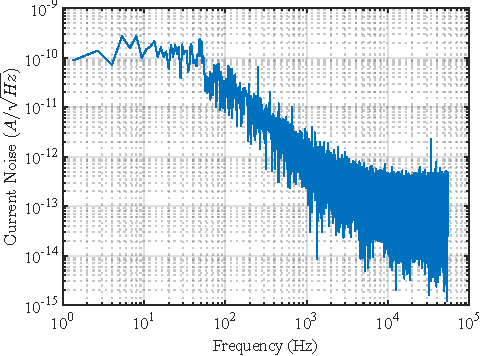
\includegraphics[width=0.9\linewidth]{4-ANC_Sys/NoiseReverseBias.pdf}
  \caption{}
  \label{fig_NoiseReverseBias}
\end{subfigure}%
\begin{subfigure}{.5\textwidth}
  \centering
  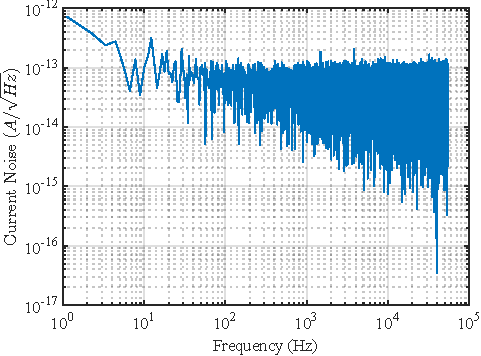
\includegraphics[width=0.9\linewidth]{4-ANC_Sys/NoiseZeroMode.pdf}
  \caption{}
  \label{fig_NoiseZeroMode}
\end{subfigure}
\caption{Light receiver board noise test with floating input (a) Reverse-bias photodiode (b) Zero mode}
\label{fig_RecBoardNoiseTest}
\end{figure}

Further testing on gain and bandwidth is made to only the zero mode configuration since it will not be practical to test and use reverse-bias configuration because of the large noise.  Before testing the board with the light circuit, we first test it with electrical input.  Fig~\ref{fig_BoardTest1khz} shows the input and output waveform when testing the new light receiver board.  The input is a \qty{23}{mV} \qty{1}{kHz} sinusoidal signal connected to the point between the photodiode and the AC coupling capacitor, via a \qty{100}{k\Omega} resistor.  This is because the photodiode outputs current, and so we need a resistor to convert the voltage input into current input.  The output is measured at the output of the two-stage low-pass filter.  From this output voltage, the gain can be calculated as:
$$Gain=\frac{V_{out}}{I_{in}}=\frac{V_{out}}{\frac{V_{in}}{R_{in}}}=\frac{\qty{1.8395}{V}}{\frac{\qty{23}{mV}}{\qty{100}{k\Omega}}}=\qty{138.06}{dB}$$

\begin{figure}[!ht]
\centering
\includegraphics[width=0.9\linewidth]{4-ANC_Sys/BoardTest1khz.png}
\caption{Board test at \qty{1}{kHz}}
\label{fig_BoardTest1khz}
\end{figure}

Fig~\ref{fig_BoardBandwidth} shows the gain at a few more frequency points.  The gain at maximum setting is at \qty{138}{dB}, which is \qty{2}{dB} lower than the \qty{140}{dB} theoretical maximum gain.  This might be caused by resistor inaccuracy, PCB track resistance and interference, or measurement error.  Overall, \qty{2}{dB} error is acceptable.  The \qty{3}{dB} bandwidth is basically the same as the simulation result, with the lower \qty{3}{dB} point at just under \qty{10}{Hz}, and the higher \qty{3}{dB} at just over \qty{10}{kHz}.  This result confirms the board is working as expected, and it meets the frequency requirement of the optrode system.

\begin{figure}[!ht]
\centering
\includegraphics[scale=0.9]{4-ANC_Sys/BoardBandwidth.pdf}
\caption{Board bandwidth test}
\label{fig_BoardBandwidth}
\end{figure}




\section{Development of the noise cancelling algorithm}

An effective noise cancelling algorithm is essential for the active noise cancelling concept to work in the optrode system.  What we want is an algorithm that is not too complex, can handle real-time input-output, and is easy to scale up to hundreds of channels.  One of the common methods for active noise cancelling is the wiener filter.  eqn~\ref{eqn_WienerMatrix} from the literature review shows how to perform the calculation for the wiener filter.  In this equation, matrix $T$ contains a symmetric Toeplitz matrix of $R_w$, which is the autocorrelation of the signal $w$.  Matrix $a$ contains the filter coefficient $a$, and matrix $v$ contains $R_{ws}$, which is the cross-correlation of the signal $w$ and the signal $s$.  We know the information in the signal $w$ and $s$, so we can calculate $R_w$ and $R_{ws}$, therefore also matrix $T$ and $v$ using the following equation:
$$R_w[m]=E\{w[n]w[n+m]\}$$
$$R_{ws}[m]=E\{w[n]s[n+m]\}$$
Where $E$ denotes the expectation operator.

From these equations, we can write code to generate filter coefficients.  However, this method uses the whole length of $w$ and $s$ and the generated coefficient $a$ has the same length.  This process takes a very long time and a lot of computational resources.  From the testing result in fig~\ref{fig_CrossCorrelationTest}, we can see that the signals are only largely correlated at 7 samples, which means there are not a lot of similarities between the two signals beyond 7 samples and we should be able to use fewer filter coefficients and achieve similar performance as the whole data length filter coefficients.  Below is a MATLAB code for a modified wiener filter function, the input is two signals $x$ and $y$, the number of filter taps, and the number of samples shifted between $x$ and $y$.  The output is $xest$ the estimated x and $FilterVector$ the filter coefficients.

\begin{lstlisting}[language=matlab]
function [FilterVector,xest] = myWiener(x,y,N,NS)
%
% Wiener filter based on Wiener-Hopf equations
%   This function takes as inputs a noisy signal, x, and a reference signal, y,
%   in order to compute a N-order linear filter that provides an estimate of y
%   from x
%  
% INPUTS
% x = noise + message signal
% y = noise signal
% N = filter order
% Ns = filter shift
%
% OUTPUTS
% xest = estimated signal
% FilterVector = Wiener filter coefficients

% Autocorrelation function
for i = 1:length(x)
    Rxx(i) = 0;
    for j = 1:length(x)
        if i + j <= (length(x) + 1)
            Rxx(i) = Rxx(i) + x(j) * x(j+i-1);
        else
            Rxx(i) = Rxx(i) + x(j) * x(j+i-length(x)-1);
        end
    end
end
% Crosscorrelation function
for i = 1:length(x)
    Rxy(i) = 0;
    for j = 1:length(x)
        if i + j <= (length(x) + 1)
            Rxy(i) = Rxy(i) + x(j) * y(j+i-1);
        else
            Rxy(i) = Rxy(i) + x(j) * y(j+i-length(x)-1);
        end
    end
end
%

Rxx = toeplitz(Rxx);
Rxy = Rxy';
B = Rxx \ Rxy;

% Create filter window centered at 1
FilterVector = zeros(1,NS-floor(N/2));
WorkingFilter = (B(NS+1-floor(N/2):NS+1-floor(N/2)+N-1))';
FilterVector = cat(2, FilterVector, WorkingFilter);

xest = filter(FilterVector,1,x);
\end{lstlisting}

------------------------------
Originally from online, modified by myself.
------------------------------

Fig~\ref{fig_TestMeasurement} shows the result of running the MATLAB code above on a set of biomedical data recorded previously.  The green $Detrend SOptrode$ is the channel that contains the cardiac signal captured with optrode, and the black $ Detrend SNoiseRef$ is the other channel that comes out from the same light source but not into an optrode.  Both of them are detrended because there has been a very slow DC level shifting because the data is captured before the capacitor on the previous receiver board has been charged up.  The red signal $Estimated Noise$ is the $Xest$ output from $myWiener$ function, and the blue signal is the green original signal subtracting the red estimated noise.  In this case, $myWiener$ function takes the input of optrode and noise reference signals and estimates a noise signal that correlates most to the optrode signal.  If we take a period of time in the flat part of the signal, i.e. from \qty{0.7}{s} to \qty{0.8}{s}, and compare the RMS value for the green and blue signal, which is the original and after process signal, we get around 30\% reduction rate.  


\begin{figure}[!ht]
\centering
\includegraphics[width=1\linewidth]{4-ANC_Sys/TestMeasurement.pdf}
\caption{TestMeasurement}
\label{fig_TestMeasurement}
\end{figure}

Now we have a working algorithm, we need to figure out how to meet the other two requirements: real-time processing, and easy to implement on FPGA.  In order to take real-time digital input sample by sample, we cannot use the whole data set, and it is not very simple to implement a moving bin algorithm on the FPGA.  Therefore, we decided to use a leaky integrator, so the weighting for each sample is at maximum when it first comes in, and gradually reduces by 0.01\% per sample.  At this rate, reducing each sample to about 5\% of the original value will require 29956 samples, which would be \qty{3}{s} at \qty{10}{kHz} sampling rate in this model.  A high-pass filter is implemented to remove the effect of DC-level shifting.  The high-pass filter block has a transfer function of $H(z)=\frac{1-Z^{-1}}{1-0.9Z^{-1}}$, at \qty{10}{kHz} sampling frequency, the cut off frequency would be around \qty{151}{Hz}.  In eqn~\ref{eqn_WienerMatrix}, if we simplify the matrix to one sample length, the filter coefficient $a$ is given by the cross-correlation of $w$ and $s$ divided by the autocorrelation of $w$.  We perform a similar process here by multiplying $NoisySignal$ and $Noise$ and integrating to get the cross-correlation, and multiplying $Noise$ by itself and integrating to get the auto-correlation, then dividing the cross-correlation to the auto-correlation to get the filter coefficient.  We multiply the $Noise$ signal by this filter coefficient to get the estimated $Noise$ signal that best matches the noise in $NoisySignal$.  Finally, subtract $NoisySignal$ by the estimated $Noise$ to get the active noise cancelling output.  This modified wiener filter structure is constructed with Simulink and shown in fig~\ref{fig_Simulink}.  The test result of this Simulink model using the same data input as the wiener filter test is shown in fig~\ref{fig_SimulinkResult}.  The blue signal is $NoisySignal$ at the input and the green signal is the output of the Simulink model.  The improvement is very close to the wiener filter result in fig~\ref{fig_TestMeasurement}, which proves this Simulink model is effective for reducing the noise in biomedical signal.

\begin{figure}[!ht]
\centering
\includegraphics[width=1\linewidth]{4-ANC_Sys/Simulink.pdf}
\caption{Simulink DSP block}
\label{fig_Simulink}
\end{figure}

\begin{figure}[!ht]
\centering
\includegraphics[width=1\linewidth]{4-ANC_Sys/SimulinkResult.pdf}
\caption{Simulink DSP Result}
\label{fig_SimulinkResult}
\end{figure}

\begin{figure}[!ht]
\centering
\includegraphics[width=1\linewidth]{4-ANC_Sys/VivadoSim.png}
\caption{Simulink DSP Result}
\label{fig_SimulinkResult}
\end{figure}



\section{DSP block}



Applications such as brain-computer interfaces (BCIs), require arrays of hundreds of optrodes working together, with all processing done in real-time with FPGAs providing the best approach for such requirements.

We used a Wiener filter~\cite{WienerFilter} for preliminary investigations on pre-recorded optrode data to verify the effectiveness of actively cancelling in a realistic setup. However, in general Wiener filters process part of the signal one bin at a time and require a large amount of computational resources when the bin size gets large.  From experimental data, the optrode system showed little correlation between data streams beyond 3 samples from zero lag. We also determined that a one-tap filter showed significant noise reduction while increasing the number of taps showed little improvement.  This is fortunate, as an algorithm that must process hundreds of channels in real time, need to be simple and consume little power.  Therefore, a one-tap adaptive filter algorithm that is based on Wiener filtering has been designed and implemented on the FPGA board.

Fig.~\ref{fig_DSP} shows the implemented digital signal processing infrastructure.  We assume here that the transfer function $H_1$ is common to both signals and that the transfer functions $H_2$ are identical integrators.  The system as shown has two inputs $x_1(i)$ and $x_2(i)$ respectively and a single output $y(i)$.  $x_1(i)$ carries the noisy message signal while $x_2(i)$ carries the noise signal.  The system is trying to remove the part of the noise in $x_1(i)$ that is correlated to the noise in $x_2(i)$, so we can posit:
$$x_1(i)=s(i)+n(i) \quad;\quad x_2(i)=m(i)+kn(i)$$
Where $n(i)$ is the part of the noise assumed present and correlated in both $x_1(i)$ and $x_2(i)$, $s(i)$ is signal plus random noise in $x_1(i)$, $m(i)$ is random noise in $x_2(i)$, and $k$ is the scale factor.  All of $s(i)$, $n(i)$, and $m(i)$ are random signals and assumed to be uncorrelated to each other.

Let $N$ be the total number of samples in $x_1(i)$ and $x_2(i)$.  Take $x_{cc}$, the cross-correlation of $x_1(i)$ and $x_2(i)$; and $x_{ac}$, the auto-correlation of $x_2(i)$, such that

$$x_{cc}(i)=\displaystyle\sum_{i=1}^{N} x_1(i)x_2(i), x_{ac}(i)=\displaystyle\sum_{i=1}^{N} x_2(i)x_2(i)$$
We divide the cross-correlation by the auto-correlation to get the filter coefficient:
\begin{equation}
\label{filterCoeff}
    \frac{x_{cc}(i)}{x_{ac}(i)} =\frac{\displaystyle\sum_{i=1}^{N} \left(s(i)m(i)+ks(i)n(i)+n(i)m(i)+n^2(i)k\right)}{\displaystyle\sum_{i=1}^{N} \left(m^2(i)+k^2n^2(i)+2km(i)n(i)\right)}
\end{equation}
Now, since $s(i)$, $n(i)$, and $m(i)$ are uncorrelated, all their respective cross-correlations should be equal to zero. In addition experiment results show that $kn(i)$ is the dominant noise in $x_2$, which means: 
$$
\sum_{i=1}^{N} k^2n^2(i) \gg \sum_{i=1}^{N} m^2(i)
$$
and consequently Eqn.~\ref{filterCoeff} reduces to:
$$
\frac{x_{cc}(i)}{x_{ac}(i)}=\frac{\displaystyle\sum_{i=1}^{N} kn^2(i)}{\displaystyle\sum_{i=1}^{N} m^2(i) + \displaystyle\sum_{i=1}^{N} k^2n^2(i)} \approx \frac{1}{k} 
$$
From this we can obtain the output $y(i)$:
\begin{align*}
    y(i)&=x_1(i)-\frac{1}{k}x_2(i) \\
    &=s(i)+n(i)-\frac{1}{k}m(i)-n(i)=s(i)-\frac{1}{k}m(i)
\end{align*}
Since $kn \gg m$, the noise level in $y$ is largely improved compared to $x_1(i)$.

To make the system more practical, a high-pass filter $H_1$ is implemented to remove any DC offset in the signals to improve cross-correlation and auto-correlation results.  A leaky integrator $H_2$ is used so the system has a moving average to track the most recent signal (in our case for about \qty{500}{ms}).  This leaky integrator compensates for the potential changes in the gain of $x_1(i)$ and $x_2(i)$ caused by {\em e.g.} temperature change or physical movement.

\begin{figure*}[htbp]
\centerline{\includegraphics[width=0.9\linewidth]{4-ANC_Sys/DataFlow.pdf}}
\caption{Data flow block diagram.  Light from a light source is split into two channels of light, one goes to the active optrode and measures nerve signal, and the other one goes to the inactive optrode and does not measure anything.  The two channels of light are then converted to digital signals and are processed by a DSP algorithm.}
\label{fig_DataFlow}
\end{figure*}

Fig.~\ref{fig_DataFlow} shows the data flows as currently implemented.  Light comes out of a light source and is split into two identical signals at the passive light splitter.  Then one signal goes to the active optrode where it measures a nerve signal, and the other signal goes to an inactive optrode and carries no extra information.  Both signals are converted into current by the photodiode, then converted into voltage by the amplifier, and finally converted into digital signals by the ADC, which all happen on the light receiver board.  Finally, the digital signals are transmitted to the FPGA for digital signal processing.

In our case, the light source is a super-luminescent diode with a \qty{1550}{\nm} wavelength, and a variable current of up to \qty{800}{\mA}, running at a constant temperature of \qty{20}{\degreeCelsius}.  The frequency range of the nerve signal is \qty{10}{\Hz} to \qty{10}{\kHz}.  The light receiver board gain is set to \qty{140}{dB\Omega} for all the measurements.  The USB serial port embedded in the FPGA board can only stream the data to a PC at 300Hz, which does not meet the requirement.  However, it is capable to stream out real-time data at \qty{64}{kHz} with suitable peripherals.  In this project, an SD card is used to store data to save development time.

\section{FPGA}

How does the FPGA board connect to the receiver board

How does the Verilog and c code work in the FPGA

\begin{figure}[!ht]
\centering
\includegraphics[width=0.9\linewidth]{4-ANC_Sys/FPGA.jpg}
\caption{FPGA}
\label{fig_FPGA}
\end{figure}

\begin{figure}[htbp]
\centerline{\includegraphics[width=1\linewidth]{4-ANC_Sys/DSP.pdf}}
\caption{Active noise cancelling algorithm block diagram.  It is an adaptive filter modified from the Wiener filter.}
\label{fig_DSP}
\end{figure}

\begin{figure}[htbp]
\centerline{\includegraphics[width=0.99\linewidth]{4-ANC_Sys/VivadoBD.pdf}}
\caption{Vivado Block Diagram}
\label{fig_VivadoBD}
\end{figure}
    %\include{4-ANC_Sys/4-1-Overview}
    %\include{4-ANC_Sys/4-2-Receiver_Board}
    %\include{4-ANC_Sys/4-3-FPGA}
    %\include{4-ANC_Sys/4-4-DSP}
    \chapter[Experiment]{Experiment result} \label{c:tc2} 

\section{Cross correlation}

\begin{figure}[H]
\centerline{\includegraphics[scale=1]{5-Experiment/Cross correlation.pdf}}
\caption{Cross correlation of active optrode and inactive optrode channel at different light source power with no input signal at the active optrode}
\label{fig_Cross correlation}
\end{figure}

For the digital signal processing algorithm to work correctly, the noise in the two light channels must be highly correlated.  By directly taking measurements from the two receiver channels without any processing algorithm, with the light source turned on and no input to the optrodes, we can calculate the cross-correlation between the channels as shown in Fig.~\ref{fig_Cross correlation}.  At low light source power, the noise of the light receiver board dominates the noise from the light source.  The biopotential signal and light source noise increase proportionally to the increase of light power, while the light receiver board noise stays the same.  When the light source current exceeds \qty{500}{\mA}, the light source noise dominates the whole noise in the system, and the normalised cross-correlation remains constant at $\sim$0.8, suggesting the possibility of active noise cancelling.

\section{Noise comparison}

Fig.~\ref{fig_500mA Signal_a} shows the captured, digitised signals before (``Active Optrode'') and after (``Noise-Cancelling Output'') the noise cancelling process is applied when the optrode input is shorted.  The Active Optrode channel clearly has a substantially larger amplitude than the Noise Cancelling Output channel.  In fig.~\ref{fig_500mA Signal_b}, a large \qty{200}{mV} sinusoidal signal is applied to the optrode.  Again, the Noise Cancelling Output channel has substantially less noise than the Active Optrode channel, confirming that the algorithm is working in the case of sinusoidal signals, even when these are much larger than the noise level.  Fig.~\ref{fig_500mA Signal_c} shows a small \qty{10}{mV} sinusoidal signal applied to the optrode.  The blue active optrode channel looks like a random signal with some high frequency noise, while the red noise cancelling output channel shows a clear periodic signal at \qty{1}{kHz}.  Although the noise cancelling output channel still has a lot of high frequency noise, it shows the ability to recover small amplitude signals from noisy active optrode channel.

\begin{figure}
\centering
\begin{subfigure}{1\textwidth}
  \centering
  \includegraphics[scale = 0.8]{5-Experiment/500mA Signal_a.pdf}
  \caption{}
  \label{fig_500mA Signal_a}
\end{subfigure}
\begin{subfigure}{1\textwidth}
  \centering
  \includegraphics[scale = 0.8 ]{5-Experiment/500mA Signal_b.pdf}
  \caption{}
  \label{fig_500mA Signal_b}
\end{subfigure}
\begin{subfigure}{1\textwidth}
  \centering
  \includegraphics[scale = 0.8 ]{5-Experiment/500mA Signal_c.pdf}
  \caption{}
  \label{fig_500mA Signal_c}
\end{subfigure}
\caption{(a) \qty{500}{\mA} light source current with zero input signal at the active optrode (b) \qty{500}{\mA} light source current with \qty{200}{\mV} peak to peak \qty{1}{\kHz} sinusoidal input signal at the active optrode (c) \qty{500}{\mA} light source current with \qty{10}{\mV} peak to peak \qty{1}{\kHz} sinusoidal input signal at the active optrode}
\label{fig_500mA Signal}
\end{figure}

\begin{landscape}\centering
\begin{figure}[h]
\centerline{\includegraphics[width=\linewidth]{5-Experiment/SimCardiac.pdf}}
\caption{\qty{500}{\mA} light source current with \qty{100}{\mV} peak to peak simulated cardiac input signal at the active optrode}
\label{fig_SimCardiac}
\end{figure}
\end{landscape}

Fig.~\ref{fig_SimCardiac} shows a simulated \qty{100}{mV} cardiac signal applied to the optrode.  This signal is similar to the cardiac signal measure from the existing optrode system that is used in Wiener filter testing (Although at a different frequency).  Compared to the blue active optrode channel, the red noise cancelling output channel shows a smoother spike and lower random noise.  

Fig.~\ref{fig_CrossCoBeforeAfterANC} shows the normalised cross correlation of the active optrode and inactive optrode channel at \qty{500}{mA} light source current, before and after the active noise cancelling process.  In fig.~\ref{fig_CrossCoBefore}, a maximum correlation of just over \qty{0.8} happens at zero lag, which matches the result measured in preliminary work with the existing optrode system.  While in fig.~\ref{fig_CrossCoAfter}, a maximum correlation of around \qty{0.4} happens at \qty{-2} lag, indicating a noise reduction in the active optrode channel, and a \qty{2} sample delay in the FPGA.  However, these two signals still have a normalised cross correlation of \qty{0.4}, implying there is still room to improve the performance. 

\begin{figure}[h]
\centering
\begin{subfigure}{.5\textwidth}
  \centering
  \includegraphics[width=0.9\linewidth]{5-Experiment/CrossCoBeforeANC.pdf}
  \caption{}
  \label{fig_CrossCoBefore}
\end{subfigure}%
\begin{subfigure}{.5\textwidth}
  \centering
  \includegraphics[width=0.9\linewidth]{5-Experiment/CrossCoAfterANC.pdf}
  \caption{}
  \label{fig_CrossCoAfter}
\end{subfigure}
\caption{Normalised cross correlation of active optrode and inactive optrode channel at \qty{500}{mA} light source current, before and after the active noise cancelling process. (a) before. (b) after. X-axis is the lag between the two samples, y-axis is the normalised correlation.}
\label{fig_CrossCoBeforeAfterANC}
\end{figure}

Fig.~\ref{fig_RMS value for ch1 and DSP output} shows the comparison between the root mean square (RMS) value for the Active Optrode channel and the Noise Cancelling Output channel for different light source currents when no voltage is applied on the optrode.  The RMS value of the Active Optrode channel (blue bars) raises when the light source current is increased showing an approximate linear relationship between the noise in the channel and the light source drive current. Similarly, the red bars show the RMS value of the Noise Cancelling Output channel. 

\begin{figure}[h]
\centerline{\includegraphics[scale=1]{5-Experiment/RMS value for ch1 and DSP output.pdf}}
\caption{Output Root-Mean-Square at different light source current with zero input signal at the active optrode}
\label{fig_RMS value for ch1 and DSP output}
\end{figure}

We can see that, at lower light source currents, the noise reduction seen in the Noise Cancelling Output channel is modest.  As the light source current increases, the noise in the Noise Cancelling Output channel grows slower than that in the Active Optrode channel, improving the relative noise reduction (i.e. the ratio between the two channels) with increasing light intensity.  The relative noise reduction plateaus at about 50\,\% noise reduction when the light source current is above \qty{500}{mA}, matching the cross-correlation result above.  Since the signal received from the optrode is ideally proportional to the light intensity (or light source drive current), we will see that the signal-to-noise ratio improvement the proposed system achieves is better at higher light source drive currents. 

\section{Optical input test with sinusoidal signal}

\begin{figure}[H]
\centerline{\includegraphics[width=1\linewidth]{5-Experiment/SNR (200mV input).pdf}}
\caption{(a) Signal-to-Noise-Ratio at different light source current with \qty{200}{\mV} peak to peak \qty{1}{\kHz} sinusoidal input signal at the active optrode (b) SNR improvement at same condition}
\label{fig_SNR (200mV input)}
\end{figure}

\begin{figure}[H]
\centerline{\includegraphics[width=1\linewidth]{5-Experiment/SNR (10mV input).pdf}}
\caption{(a) Signal-to-Noise-Ratio at different light source current with \qty{10}{\mV} peak to peak \qty{1}{\kHz} sinusoidal input signal at the active optrode (b) SNR improvement at same condition}
\label{fig_SNR (10mV input)}
\end{figure}

Fig.~\ref{fig_SNR (200mV input)} and fig.~\ref{fig_SNR (10mV input)} show the signal-to-noise ratio and signal-to-noise ratio improvement before and after the active noise cancelling process, for \qty{200}{mV} and \qty{10}{mV} sinusoidal inputs applied to the optrode, at different light source currents.  There is an outlying data point at the \qty{300}{mA} light source current, but overall the data matches the previous result that (i) at lower light source currents the signal-to-noise ratio improvement is modest, (ii) as the light source current increases, the signal-to-noise ratio improvement increases and (iii) as the light source drive current exceeds \qty{500}{mA}, the signal-to-noise ratio improvement plateaus. The power spectral density plots in Fig.~\ref{fig_Periodogram 500mA (10mV input)} shows a comparison of the Active Optrode channel (a) and Noise Cancelling Output channel (b) at \qty{500}{mA} light current with a \qty{10}{\mV}, \qty{1}{\kHz} sinusoidal signal applied at the active optrode.  The \qty{1}{\kHz} signal level in both graphs stays the same, while the noise floor magnitude drops by \qty{5}{dB} to \qty{10}{dB} in the Noise cancelling Output channel, matching the results from previous readings.

\begin{figure}[H]
\centerline{\includegraphics[width=1\linewidth]{5-Experiment/Periodogram 500mA (10mV input).pdf}}
\caption{(a) Periodogram of active optrode channel at \qty{500}{\mA} light source current with \qty{10}{\mV} peak to peak \qty{1}{\kHz} sinusoidal input signal at the active optrode (b) Periodogram of noise cancelling output channel at \qty{500}{\mA} light source current with \qty{10}{\mV} peak to peak \qty{1}{\kHz} sinusoidal input signal at the active optrode}
\label{fig_Periodogram 500mA (10mV input)}
\end{figure}

\section{Physical movement artefacts}

When mounting the nerve signal detection device on a subject, optrode systems commonly suffer artifacts due to physical movements between the system and the subject.  These artifacts are largely caused by the deformation of light fibres, and can add a significant amount of noise to the captured signals.  Since both light channel circuits are mounted in close proximity, the artifacts showing in both channels are similar.  Therefore, our active noise cancelling system is able to significantly reduce the movement-induced artifacts.  Fig.~\ref{fig_Movement Artifact} shows the result of an experiment where the light receiver board was moved while capturing data with a zero input at the active optrode.  The Active Optrode channel clearly shows substantial noise induced by movement.  Although there is still some low-frequency noise left in the Noise Cancelling Output channel, it is evident that the movement-induced noise has been largely removed.

\begin{figure}[h]
\centerline{\includegraphics[scale=1]{5-Experiment/Movement Artifact.pdf}}
\caption{Movement induced artifacts and artifact removal at \qty{500}{\mA} light source current with a zero input signal to the active optrode}
\label{fig_Movement Artifact}
\end{figure}


    %\chapter{Introduction}


\section{Optrode System}

\begin{figure}[htbp]
\centerline{\includegraphics[width=0.9\linewidth]{OptrodeFigure.pdf}}
\caption{(a) Diagram of optrode transducer used in electrophysiological  detection.  Light comes in from Polarization-maintaining (PM) fibre, is rotated by liquid crystal, reflected by the mirror and goes back into the PM fibre. (b) Optrode electrophysiological  detection system block diagram.  Light goes into the optrode from the light source, carries nerve signal, and is converted at the receiver board and DAQ to digital signal.}
\label{fig_OptrodeFigure}
\end{figure}

An optical-electrode or ``optrode'' is a recently developed device for detecting biopotential signals of neuronal, cardiac, or muscular origin.~\cite{OptrodeTransducer}.  Fig.~\ref{fig_OptrodeFigure}(a) shows the structure of such an optrode: light that is generated from a super-luminescent diode light source is guided to the optrode via a polarisation-maintaining fibre (PM fibre).  The polarised light sees its polarisation being rotated by a thin (5\ $\mu$m) layer of liquid crystals by an angle depending on the voltage applied across the metal contacts~\cite{LCVsensor}.  The light is then reflected by the back mirror and returns to the PM fibre where the amount of light recaptured depends on the rotation angle of the liquid crystals. The optrode is designed to create a linear relationship between the light detected and the voltage applied to the metal contacts.

In an existing electrophysiological  detection system such as sketched in Fig.~\ref{fig_OptrodeFigure}(b), the optrode is used to convert neuronal signals into light signals as explained above.  The light intensity recaptured is -- in this case -- modulated by the biopotential signal present at one of the metal contacts (the other one being grounded). The light that comes out from the optrode is then directed to a receiver board where a photodiode converts the light into an analogue electrical signal which is then sampled by the data acquisition equipment.

This system has lower signal attenuation~\cite{OptrodeArray,ImpedanceOfOptrode} compared to conventional electronic detection systems. However, the output noise level of the current system is significantly higher than that of conventional microelectrode-based systems. This means it is harder to observe nerve activity, especially when the signal amplitude is small (less than~\qty{10}{mV}).  In previous experiments, it was observed that most of the noise was coming from the light source and thus, a direct way to reduce noise is to design a low-noise current source~\cite{LowNoiseCurrentSource} to power the light source.  In this paper, we propose an additional method to reduce noise: active noise cancelling.

The active noise cancelling technique is used in multiple applications such as noise-cancelling headphones~\cite{ANC_Headphone_1,ANC_Headphone_2}, noise-cancelling in cars~\cite{ANC_Car}, RF signal noise-cancelling~\cite{ANC_RF}, {\em etc}.  The basic principle of active noise cancelling for the sound wave is that when two waves have basically the same frequency and amplitude but opposite phases, they will cancel each other out.  In our case, we are dealing with noise in the digital signal form, which requires filtering techniques rather than just subtracting the two signals.  Wiener filters~\cite{WienerFilter} are widely used in signal processing of active noise cancelling applications {\em e.g.}\cite{ANC_Wiener_2,ANC_Wiener_3}.  Since the nerve signal that the optrode system is detecting has a similar frequency range compared to audible sound frequency, active noise cancelling with Wiener filtering should be effective here as well. Thus we propose herein such an approach which, to the best of our knowledge, has not yet been proposed elsewhere.


\section{Scope of work}

This project aims at designing a active noise cancelling system that reduces the noise level in an existing optrode measurement system. The main outcome of this project is the active noise cancelling system that consists of two board, a light receiver PCB, and an FPGA development board. The project begins with a literature review to active noise cancelling designs, and optrode.  Then we analyzes previous receiver boards and designs a new light receiver board, simulation are run and performance are tested to ensure the circuits on the board work as expected. The heart of the project lies in the development of a noise-cancelling algorithm, starting with the foundational Wiener filter. This filter is then modified and tested first in MATLAB, and then implemented in Verilog HDL, with further explorations into the usage of DSP blocks and final implementation on an FPGA platform.  Experimental sections examine the correlation between different noise signals, compare the performance of the newly designed system with existing technologies, test with sinusoidal signals on optical input, and study the artifacts introduced by physical movements and their impact on signal quality.

    \chapter{Conclusion and Future Directions}\label{c:conclusion}

\subsection{Future work}

To be able to work with an optrode array with hundreds of channels, the filter implementation needs to be optimised by reducing the resolution in the algorithm (just enough for subsequent usage), or time-share resources, so that hundreds of filter channels can fit in the processing unit.  Alternatively, while our design focus has been on multiple-optrode arrays, the proposed method is equally applicable in systems with few optrodes;  for such systems, filter resource use is of less concern and a more complex filter algorithm with more taps can be designed to achieve the full potential of active noise cancelling~\cite{ANCHeadphone}.

\subsection{Conclusion}

In this project, we demonstrate experimentally for the first time an active noise cancelling technique in an optrode detection system. This system uses an active optrode to record signals and an inactive optrode to estimate noise. A light receiver board is designed and assembled that converts the two channels of light into digital signals, and an adaptive digital filter is designed and run on an FPGA board that is used to reduce the noise in the signal channel. The system reduces the noise in the optrode system by up to 50\% and is capable of reducing artifacts from physical movements.
   
    \clearpage
   
    %appendices
    \appendix
    \chapter[Appendix: a]{Verilog and C codes}\label{a:codes}

\lstinputlisting[language=matlab]{8-appendices/Codes/myWiener.m}
\lstinputlisting[language=matlab]{8-appendices/Codes/test_measurement.m}

\lstinputlisting[language=c]{8-appendices/Codes/helloworld.c}

\lstinputlisting[language=verilog]{8-appendices/Codes/128_CLK_divider.v}
\lstinputlisting[language=verilog]{8-appendices/Codes/Debouce.v}
\lstinputlisting[language=verilog]{8-appendices/Codes/Debounce_2bits.v}
\lstinputlisting[language=verilog]{8-appendices/Codes/Debounce_4bits.v}
\lstinputlisting[language=verilog]{8-appendices/Codes/Delay.v}
\lstinputlisting[language=verilog]{8-appendices/Codes/DSP_2dot1V.v}
\lstinputlisting[language=verilog]{8-appendices/Codes/DSP_24to64.v}
\lstinputlisting[language=verilog]{8-appendices/Codes/DSP_64to24.v}
\lstinputlisting[language=verilog]{8-appendices/Codes/FIFO_Buffer.v}
\lstinputlisting[language=verilog]{8-appendices/Codes/SPI_ADC_read_loop.v}
\lstinputlisting[language=verilog]{8-appendices/Codes/SPI_Controller_2.v}
\lstinputlisting[language=verilog]{8-appendices/Codes/SPI_MASTER.v}
\lstinputlisting[language=verilog]{8-appendices/Codes/SPI_Master_CS.v}


\lstinputlisting[language=verilog]{8-appendices/Codes/Adder.v}
\lstinputlisting[language=verilog]{8-appendices/Codes/Adder_32bit.v}
\lstinputlisting[language=verilog]{8-appendices/Codes/bit64_adder.v}
\lstinputlisting[language=verilog]{8-appendices/Codes/bit64_delay.v}
\lstinputlisting[language=verilog]{8-appendices/Codes/bit64_divide_64by64.v}
\lstinputlisting[language=verilog]{8-appendices/Codes/bit64_multiply_0dot9.v}
\lstinputlisting[language=verilog]{8-appendices/Codes/bit64_multiply_0dot9999.v}
\lstinputlisting[language=verilog]{8-appendices/Codes/bit64_multiply_1.v}
\lstinputlisting[language=verilog]{8-appendices/Codes/bit64_multiply_64by64.v}
\lstinputlisting[language=verilog]{8-appendices/Codes/bit64_multiply_minus1.v}
\lstinputlisting[language=verilog]{8-appendices/Codes/bit64_subtract.v}
\lstinputlisting[language=verilog]{8-appendices/Codes/clk_rst_gen.v}
\lstinputlisting[language=verilog]{8-appendices/Codes/Delay_1_16bit.v}
\lstinputlisting[language=verilog]{8-appendices/Codes/Delay_1_32bit.v}
\lstinputlisting[language=verilog]{8-appendices/Codes/Divide_16_bit.v}
\lstinputlisting[language=verilog]{8-appendices/Codes/Divide_32bit_to_16bit.v}
\lstinputlisting[language=verilog]{8-appendices/Codes/Multiply_0dot9_16bit.v}
\lstinputlisting[language=verilog]{8-appendices/Codes/Multiply_0dot9999_32bit.v}
\lstinputlisting[language=verilog]{8-appendices/Codes/Multiply_1_16bit.v}
\lstinputlisting[language=verilog]{8-appendices/Codes/Multiply_2_16bit.v}
\lstinputlisting[language=verilog]{8-appendices/Codes/Multiply_3_16bit.v}
\lstinputlisting[language=verilog]{8-appendices/Codes/Multiply_16bit_by_16bit.v}
\lstinputlisting[language=verilog]{8-appendices/Codes/Multiply_16by16_16out.v}
\lstinputlisting[language=verilog]{8-appendices/Codes/Nand.v}
%\lstinputlisting[language=verilog]{8-appendices/Codes/Step_input.v}
\lstinputlisting[language=verilog]{8-appendices/Codes/Subtract_16bit.v}


\lstinputlisting[language=tcl]{8-appendices/Codes/Arty-Z7-20-Master.xdc}


Code used from nandland












    \chapter{Documentation}\label{a:documentation}


   
    \clearpage
    
    \backmatter
    
    \pagestyle{noHeading}
    \bibliographystyle{IEEEtran}
    \bibliography{references}

\end{document}
